\documentclass[12pt,aspectratio=169]{beamer}

\usetheme{metropolis}

\definecolor{mDarkBrown}{HTML}{FF5722}
\definecolor{mDarkTeal}{HTML}{263238}
\definecolor{mLightBrown}{HTML}{FF5722}

\usepackage{graphicx}
\usepackage{hyphenat}

\usepackage{minted}
\usemintedstyle{tango}
\newminted[py3]{python}{%
    python3,
    autogobble,
    bgcolor=mDarkTeal!10,
    linenos
}

\usepackage{polyglossia}
\setdefaultlanguage[variant=british]{english}
\usepackage[english=british]{csquotes}

\defaultfontfeatures{Ligatures=TeX}
\setmainfont{Lucida Sans OT}
\setsansfont[Scale=MatchLowercase]{Lucida Sans OT}
\setmonofont[Scale=MatchLowercase]{Lucida Console DK}

\author{Gianluca Campanella}
\date{}



\title{Python Programming 101}

\begin{document}

\maketitle

\begin{frame}{Today's class}
    \begin{block}{Prerequisites}
        \begin{itemize}
            \item No previous programming experience required
            \item Lots of slides with \mintinline{python}{actual code}
        \end{itemize}
    \end{block}
    \vfill
    \begin{block}{Goals}
        \begin{itemize}
            \item Make you self\hyp{}sufficient as a Python beginner
            \item Teach you a little bit about Python's culture
        \end{itemize}
    \end{block}
\end{frame}

\begin{frame}[fragile]{Why Python?}
    \begin{block}{Ideal for scripting and rapid prototyping}
        \begin{itemize}
            \item General\hyp{}purpose, high\hyp{}level language
            \item Elegant syntax
            \item Interpreted
            \item `Comes with batteries' (lots of them!)
            \item The Zen of Python: \mintinline{python}{import this}
        \end{itemize}
    \end{block}
\end{frame}

\begin{frame}{Python 2 vs Python 3}
    \begin{block}{There are two Pythons!}
        \begin{itemize}
            \item Currently: Python 2.7 and Python 3.6
            \item Minimal differences for beginners
                  (except \mintinline{python}{print})
            \item `Python 2.x is legacy, Python 3.x is the present and future of
                   the language'
        \end{itemize}
    \end{block}
\end{frame}

\begin{frame}{Let's install Python!}
    \begin{center}
        \Large%
        Download Anaconda from \\[\medskipamount]
        \url{https://www.anaconda.com/download/}
    \end{center}
\end{frame}

\begin{frame}{Using Python}
    \begin{itemize}
        \setlength{\itemsep}{0.75em}
        \item (I)Python interpreter
        \item Scripts
        \item Jupyter (previously IPython) Notebooks
    \end{itemize}
\end{frame}

\begin{frame}[fragile]{REPL}
    \begin{itemize}
        \item \textbf{R}ead some input
        \item \textbf{E}valuate
        \item \textbf{P}rint the result
        \item \textbf{L}oop (i.e.\ repeat)
    \end{itemize}
    \vfill
    \begin{center}
        Let's try it now: what is \mintinline{python}{2 + 2}?
    \end{center}
\end{frame}

\begin{frame}[fragile]{Python as a calculator}
    \begin{py3}
        1 + 2    # Addition
        3 - 4    # Subtraction
        5 * 6    # Multiplication
        7 / 8    # Division (integer division in Python 2)
        7 // 8   # Integer division
        9 ** 10  # Exponentiation
        11 % 10  # Modulo
    \end{py3}
\end{frame}

\begin{frame}[fragile]{Careful with operator precedence!}
    \begin{py3}
        1 + 2 ** 3 * 4
        1 + (2**3) * 4
        1 + ((2**3) * 4)
        ((1) + (((2)**(3)) * (4)))  # Don't overdo it! :-)
    \end{py3}
\end{frame}

\section{Variables and operators}

\begin{frame}[fragile]{Variables}
    Variables store values of different \alert{types}:
    \begin{itemize}
        \item \mintinline{python}{bool}eans are either \mintinline{python}{True}
              or \mintinline{python}{False}
        \item \mintinline{python}{int}egers are whole numbers
        \item \mintinline{python}{float}ing point are decimal numbers
        \item \mintinline{python}{str}ings are sequences of characters
        \item \mintinline{python}{None}
    \end{itemize}
    \vfill
    \begin{py3}
        session = 'Introduction to Python'  # Or use "..."
        day = 26
        temperature = 21.2
        pressure = 7.6e2  # Same as 7.6 * 10**2 = 760
    \end{py3}
\end{frame}

\begin{frame}[fragile]{Working with variables}
    \begin{py3}
        temp_c = 21.2
        temp_f = temp_c * 1.8 + 32
    \end{py3}
    \vfill\pause
    \begin{block}{Changing type (`casting')}
        \begin{py3}
            int('26')
            str(21.2)
            float('21,2')  # Oops...
        \end{py3}
    \end{block}
\end{frame}

\begin{frame}[fragile]{Operators}
    \begin{itemize}
        \setlength{\itemsep}{0.75em}
        \item Assignment: \mintinline{python}{=}
        \item Comparison: \mintinline{python}{==}, \mintinline{python}{!=},
                          \mintinline{python}{<}, \mintinline{python}{<=},
                          \mintinline{python}{>}, \mintinline{python}{>=}
        \item Mathematical: \mintinline{python}{+}, \mintinline{python}{-},
                            \ldots
        \item Logical: \mintinline{python}{and}, \mintinline{python}{or},
                       \mintinline{python}{not}
    \end{itemize}
    \vfill
    \begin{py3}
        1 + 2
        1 < 2
        'Lon' + 'don'
        'Lon' < 'don'
    \end{py3}
\end{frame}

\section{Data structures}

\begin{frame}[fragile]{Lists}
    \begin{itemize}
        \item Lists are \alert{ordered sequences} of items
              (so are \mintinline{python}{str}ings!)
        \item Not necessarily of the same type
    \end{itemize}
    \vfill
    \begin{py3}
        a = [0, 1, 1, 2, 3, 5, 8, 13, 21, 34]
        b = ['I', 'love', 'Python!']
        a + b
    \end{py3}
\end{frame}

\begin{frame}[fragile]{Tuples}
    \begin{itemize}
        \item Tuples are similar to lists, but \alert{immutable}
        \item Not necessarily of the same type
    \end{itemize}
    \vfill
    \begin{py3}
        a = (0, 1, 1, 2, 3, 5, 8, 13, 21, 34)
        b = ('I', 'love', 'Python!')
        a + b
    \end{py3}
\end{frame}

\begin{frame}[fragile]{Indexing and slicing}
    \begin{columns}
        \begin{column}{0.2\textwidth}
            \begin{py3}
                a[0]
                a[1]
                a[-2]
                a[3:]
                a[:4]
                a[5:7]
                a[::2]
            \end{py3}
        \end{column}
        \begin{column}{0.8\textwidth}
            \begin{center}
                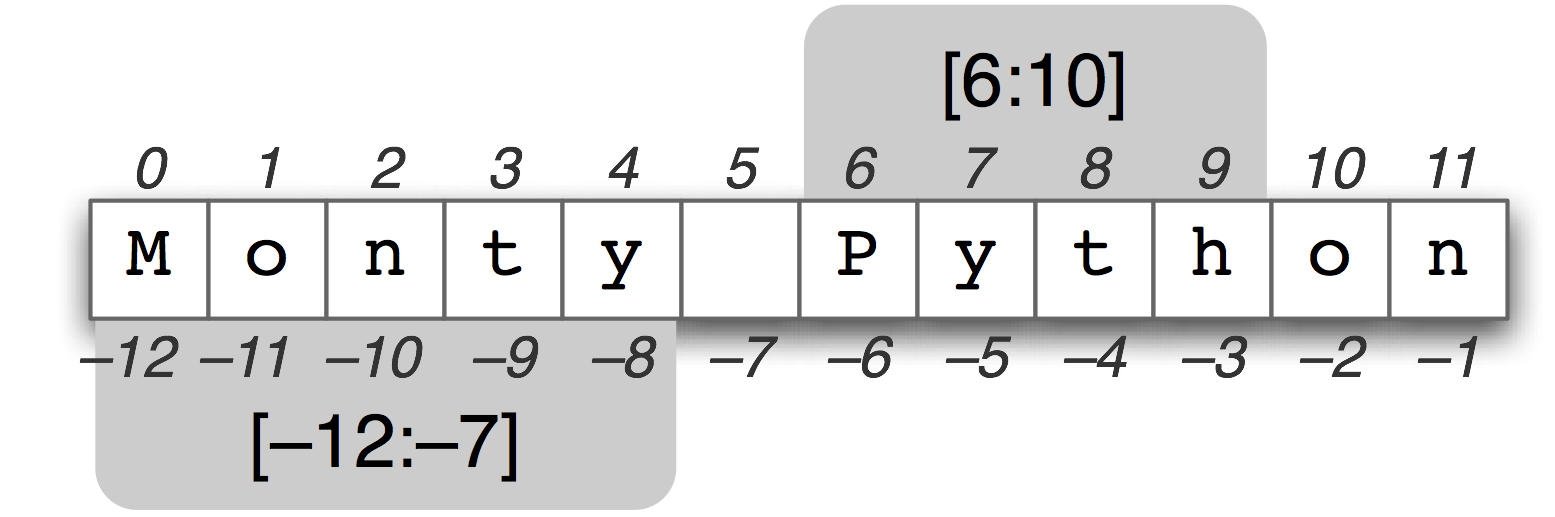
\includegraphics[width=\textwidth]{figures/py_str} \\
                {\scriptsize%
                 From \textit{Natural Language Processing with Python}}
            \end{center}
        \end{column}
    \end{columns}
\end{frame}

\begin{frame}[fragile]{Dictionaries}
    \begin{itemize}
        \item Dictionaries store \alert{key--value pairs}
        \item (Not necessarily of the same type)
    \end{itemize}
    \vfill
    \begin{py3}
        john = {
            'first_name': 'John',
            'last_name': 'Doe',
            'age': 32
        }
        john['age']
        list(john.keys())
        list(john.values())
    \end{py3}
\end{frame}

\section{Flow control}

\begin{frame}[fragile]{`If' statements}
    \begin{itemize}
        \item One \mintinline{python}{if} followed by a condition
        \item Zero or more \mintinline{python}{elif}s (short for 'else if')
        \item Optionally a final \mintinline{python}{else}
    \end{itemize}
    \vfill
    \begin{py3}
        if x < 0:
            print('x is negative')
        elif x == 0:
            print('x is zero')
        else:
            print('x is positive')
    \end{py3}
\end{frame}

\begin{frame}[fragile]{`For' loops}
    \begin{columns}
        \begin{column}{0.5\textwidth}
            \begin{py3}
                for x in range(10):
                    if x == 3:
                        continue
                    elif x == 5:
                        break
                    print(x)
            \end{py3}
        \end{column}
        \begin{column}{0.5\textwidth}
            \begin{center}
                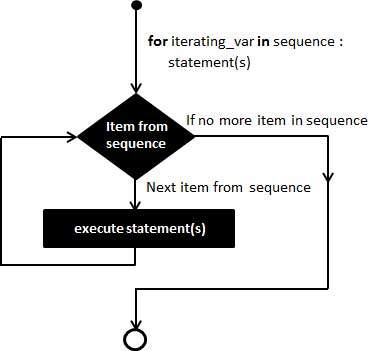
\includegraphics[height=0.75\textheight]{figures/for_loop} \\
                {\scriptsize%
                 From \textit{TutorialsPoint.com}}
            \end{center}
        \end{column}
    \end{columns}
\end{frame}

\begin{frame}[fragile]{`For' loops with lists}
    \begin{py3}
        a = ['one', 'two', 'three', 'four', 'five']

        for value in a:
            print(value)

        for index, value in enumerate(a):
            print('Item {} is "{}"'.format(index, value))
    \end{py3}
\end{frame}

\begin{frame}[fragile]{List comprehensions}
    \begin{py3}
        a = [0, 1, 2, 3, 4, 5]
        b = []

        for x in a:
            if x > 0:
                b.append(x**2)
    \end{py3}
    \vfill
    \begin{py3}
        a = [0, 1, 2, 3, 4, 5]
        b = [x**2 for x in a if x > 0]
    \end{py3}
\end{frame}

\begin{frame}[fragile]{`For' loops with dictionaries}
    \begin{py3}
        a = {
            'one': 'uno',
            'two': 'due',
            'three': 'tre',
            'four': 'quattro',
            'five': 'cinque'
        }

        for key, value in a.items():
            print('"{}" maps to "{}"'.format(key, value))
    \end{py3}
\end{frame}

\begin{frame}[fragile]{`While' loops}
    \begin{columns}
        \begin{column}{0.5\textwidth}
            \begin{py3}
                x = 0
                while x < 10:
                    x += 1
                    print(x)
            \end{py3}
            \vfill
            \begin{py3}
                x = 0
                while True:
                    if x == 10:
                        break
                    x += 1
                    print(x)
            \end{py3}
        \end{column}
        \begin{column}{0.5\textwidth}
            \begin{center}
                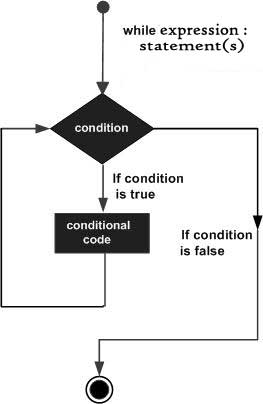
\includegraphics[height=0.75\textheight]{figures/while_loop} \\
                {\scriptsize\em%
                 From \textit{TutorialsPoint.com}}
            \end{center}
        \end{column}
    \end{columns}
\end{frame}

\section{Functions and libraries}

\begin{frame}[fragile]{Functions}
    \begin{block}{Functions\ldots}
        \begin{itemize}
            \item Take input \alert{arguments}
            \item Execute statement(s)
            \item \mintinline{python}{return} output
            \item (Not necessarily of the same type)
        \end{itemize}
    \end{block}
    \vfill
    \begin{columns}
        \begin{column}{0.5\textwidth}
            \begin{py3}
                def multiply(a, b):
                    return a * b

                multiply(2, 3)
            \end{py3}
        \end{column}
        \begin{column}{0.5\textwidth}
            \begin{py3}
                def greet(name):
                    print('Hello ' + name)

                greet('John')
            \end{py3}
        \end{column}
    \end{columns}
\end{frame}

\begin{frame}[fragile]{Libraries}
    \begin{block}{Libraries are\ldots}
        \begin{itemize}
            \item Reusable collections of code that someone else (or you) has
                  already written
            \item Part of the Standard Library
                  (e.g.\ \mintinline{python}{random})
            \item Distributed through PyPI -- the Python Package Index
                  (e.g.\ \mintinline{python}{pandas})
        \end{itemize}
    \end{block}
    \vfill
    \begin{columns}
        \begin{column}{0.5\textwidth}
            \begin{py3}
                import random

                random.randint(1, 100)
            \end{py3}
        \end{column}
        \begin{column}{0.5\textwidth}
            \begin{py3}
                from random import randint

                randint(1, 100)
            \end{py3}
        \end{column}
    \end{columns}
\end{frame}

\section{Making coding more enjoyable}

\begin{frame}{Making coding more enjoyable}
    \only<1>{%
        \begin{block}{Write short lines}
            \begin{itemize}
                \item Don't pack too much in a single long line
                      (historically: 80 characters)
                \item Clever one\hyp{}liners don't make you smarter
                \item Karma: the next person to read your code will hate you
            \end{itemize}
        \end{block}}
    \only<2>{%
        \begin{block}{Write short functions}
            \begin{itemize}
                \item If it doesn't fit on screen, break it down
                \item Think in a modular way
                      (giving birth to programs is painful)
                \item Write reusable code and don't repeat yourself
            \end{itemize}
        \end{block}}
    \only<3>{%
        \begin{block}{Choose meaningful names}
            \begin{itemize}
                \item For both functions and variables
                \item Make the purpose clear
                \item The code should be the documentation\ldots~but write the
                      documentation too
            \end{itemize}
        \end{block}}
    \only<4>{%
        \begin{block}{Rewrite and polish often}
            \begin{itemize}
                \item Understand and accept that you will make mistakes
                \item There is no royal road to coding
                \item `Negative lines of code'
            \end{itemize}
        \end{block}}
\end{frame}

\end{document}

